\namedchapter{Projekt elektroniki}
Podstawowym zadaniem projektu jest budowa robota mobilnego, na którą składa się część mechaniczna, elektroniczna oraz programowa. Pierwsza z nich została omówiona w poprzednim rozdziale. Następnym krokiem jest zaprojektowanie oraz wykonanie części wykonawczej, która pozwoli połączyć platformę \textit{Raspberry Pi} z rzeczywistym modelem i umożliwi sterowanie nim. 
\namedsection[Adam Zieliński]{Założenia}
Sterowanie pojazdem odbywa się poprzez wykorzystanie dwóch silników \textit{Pololu 37Dx52L} oraz dwóch serwomechanizmów \textit{TowerPro SG-5010}. Każdy z nich sterowany jest przy pomocy sygnału PWM (ang. \textit{Pulse-Width Modulation}), czyli sygnału prostokątnego o zmiennym współczynniku wypełnienia, co zostało pokazane na rysunku \ref{sygnal_PWM}. Aby jak najbardziej zoptymalizować proces sterowania należało wykorzystać sprzętowe generatory sygnału PWM. W odróżnieniu od programowych rozwiązań, nie obciąża to pracy procesora. Jest to o tyle istotne ,iż głównym zadaniem czołgu jest analiza obrazu pochodzącego z kamery w czasie rzeczywistym, co jest bardzo czasochłonnym procesem. Wybrana platforma \textit{Raspberry Pi} posiada dwa sprzętowe kanały PWM, z czego jeden przeznaczony jest do generowania sygnału audio. Z pojedynczego źródła możliwe jest wytworzenie dwóch przebiegów, o tej samej częstotliwości lecz różnym wypełnieniu, które posłużą do sterowania położeniem wieżyczki. Sterowanie silnikami napędowymi wymaga użycia jeszcze dodatkowo czterech sygnałów PWM. W związku z czym zaprojektowany został osobny układ elektroniczny, który pozwolił na ich obsługę. Zbudowany został w oparciu o dwa mikrokontrolery z rodziny AVR, łączące się przy pomocy magistrali szeregowej magistrali TWI(ang. \textit{2-wire Serial Interface}) z \textit{Raspberry Pi}. Komunikacja z robotem będzie wykorzystać sieć WLAN(ang. \textit{Wireless Local Area Network,}) oraz protokoł SSH (ang. \textit{secure shell}). Schemat blokowy elektroniki czołgu przedstawiony został na rysunku poniżej:

  \begin{figure}[H]
    \begin{center}
      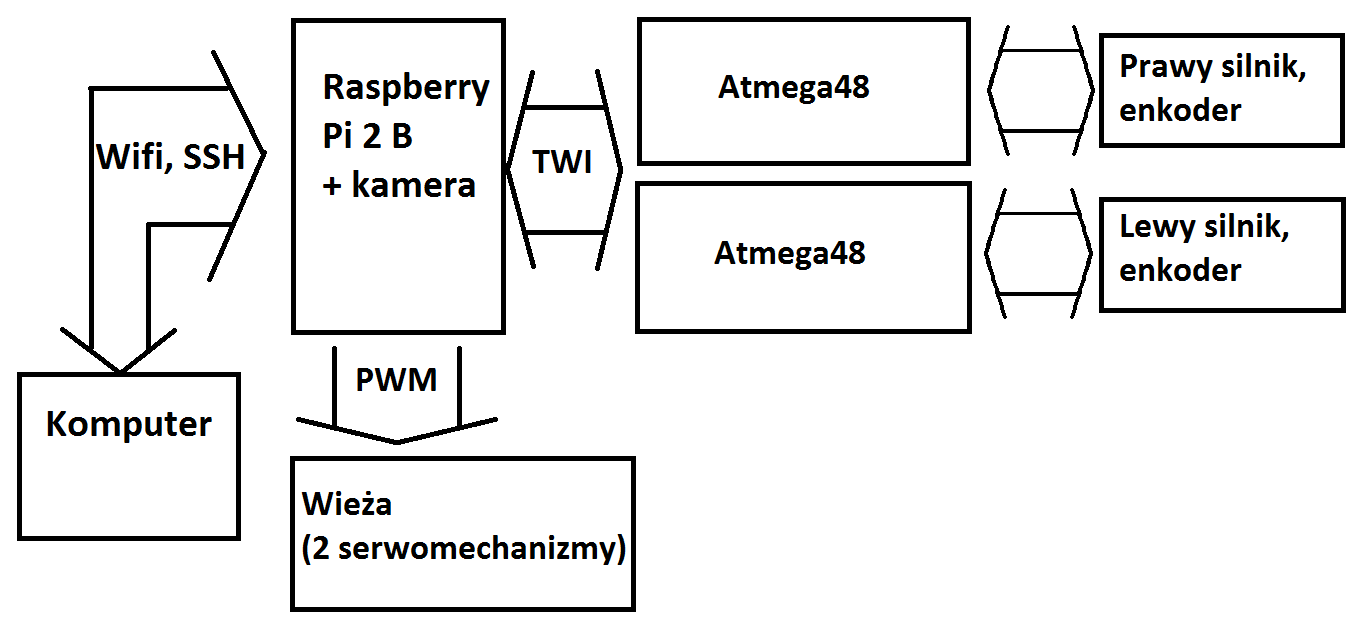
\includegraphics[scale=0.35]{imgs/idea.png}
 	\caption[Koncepcja elektroniki.]{\small{Ogólna koncepcja elektroniki pojazdu.}}
	\label{sygnal_PWM}
    \end{center}
  \end{figure}  
  
\namedsection[Adam Zieliński]{Raspberry Pi}
\textit{Raspberry Pi 2 model B} jest w minikomputerem zbudowanym w oparciu o procesor ARM Cortex-A7. Wyposażony jest w 4 porty USB (ang. \textit{Universal Serial Bus}) oraz port HDMI (ang. \textit{High Definition Multimedia Interface}) co pozwala na podłączenie monitora, klawiatury oraz myszki i czyni go w pełni funkcjonalnym komputerem. Dodatkowo istnieje możliwość zainstalowania na jego pokładzie specjalnej odmiany systemu Linux - Raspbiana, która jest zoptymalizowana i dostosowana do uwarunkowań sprzętowych \textit{Raspberry Pi}. Pozwala ona obsługę urządzenia przy pomocy wiersza poleceń oraz graficznego interfejsu użytkownika. Omawiane urządzenie łączy w sobie uniwersalność komputera klasy PC oraz mikrokontrolera. Płytka wyposażona jest w 40 pinów ogólnego przeznaczenia zapewniających m.in. komunikację TWI, generowanie sygnałów PWM czy dowolna programowa obsługa pozostałych wejść/wyjść. System operacyjny dodatkowo zawiera w sobie narzędzia niezbędne do pisania programów wykorzystujących jego sprzętowe zasoby zarówno w języku C++ jak i Pythonie. 

\begin{figure}[H]
    \begin{center}
      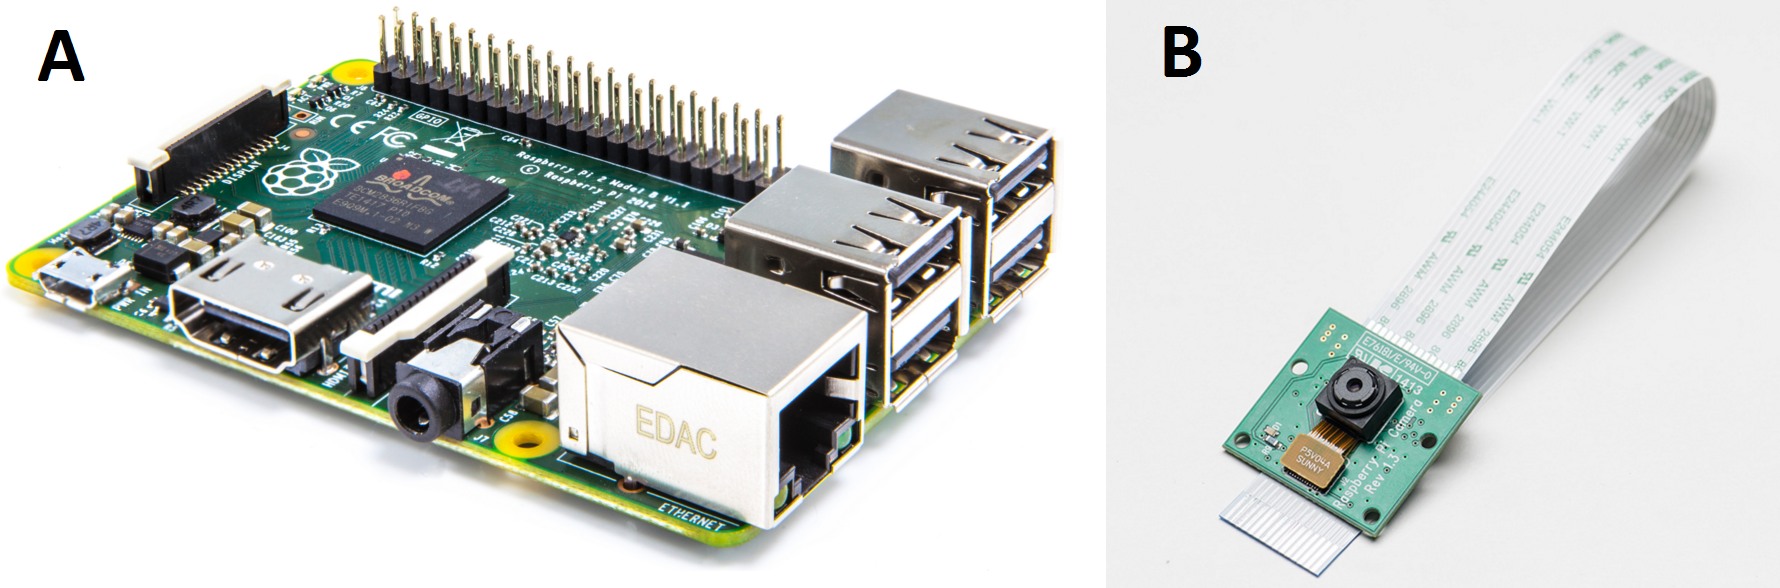
\includegraphics[scale=0.3]{imgs/raspberry_pi.png}
 	\caption[Raspberry Pi wraz z kamerą.]{\small{Na zdjęciu przedstawione zostało: A - \textit{Raspberry 2 Pi Model B}}\footnotemark \small{, B - dedykowana kamera \textit{Raspberry Pi Camera HD}}\footnotemark }
	\label{trans_TWI}
    \end{center}
  \end{figure}  
  	  \footnotetext[1]{\emph{Pi2ModB1GB}, http://raspberrypi.org/,  (data dostępu 27.12.2015 r.)}
  	  \footnotetext{\emph{RaspberryPi camera}, http://parallella.org/,  (data dostępu 27.12.2015 r.)}

Realizowany projekt inżynierski wykorzystuje wspomniany układ do realizacji analizy obrazu, które pozyskiwane są przez dedykowaną kamerę - \textit{Raspberry Pi Camera HD}. Kamera łączy się z minikomputerem przy wykorzystaniu interfejsu CSI (ang. \textit{Camera Serial Interface}) prowadzonego przy pomocy 15-pinowej taśmy. Tym co odróżnia CSI od innych popularnych interfejsów szeregowych (np. USB) jest to, że zapewnia większą przepustowość danych. Wykorzystana tutaj komunikacja składa się z: interfejsu I$^2$C, którym przesyłane są sygnały sterujące pracą kamery, dwóch dodatkowych szyn danych przeznaczonych do przesyłania obrazu oraz synchronizującej je szyny zegarowej. 
Budowany pojazd jest robotem mobilnym, co uniemożliwia podłączenie do niego monitora oraz klawiatury na stałe. Istnieje jednak możliwość w pełni funkcjonalnej, zdalnej łączności z textit{Raspberry Pi} z poziomu komputera osobistego. Do tego calu należy wyposażyć minikomputer w adapter WLAN, aby mógł połączyć się z bezprzewodową siecią lokalną do której podłączony jest także komputer osobisty. Raspbian umożliwia obsługę protokołu SSH  czyli realizację połączenia typu serwer-klient, do której obsługi wystarczy jedynie znajomość adresu IP (ang. \textit{Internet Protocol Address}) \textit{Raspberry}.
  
\namedsection[Adam Zieliński]{Sterowanie napędem}
Do napędzenia pojazdu użyte zostały szczotkowe silniki prądu stałego firmy Pololu, których ideowa konstrukcja została pokazana poniżej (rys. \ref{silnik_p}). Obrót wału silnika spowodowany jest wystąpieniem siły elektromotorycznej $F$, czyli siły działającej na przewód o długości $L$, przez który płynie prąd $I$, znajdujący się w polu magnetycznym o indukcji $B$ definiowanej jako:
\begin{equation}
	F =  BIL
   \label{eq:sila_elektromotoryczna}
 \end{equation}
 gdzie:  
 \begin{equationDescriptor}
   \EQDitem{$F$}{siła [N],}
 	\EQDitem{$B$}{indukcja magnetyczna [T],}
 	 \EQDitem{$I$}{natężenie prądu [A],}
 	  \EQDitem{$L$}{długość przewodu [m].}
 \end{equationDescriptor}
 \newpage
  \begin{figure}[H]
    \begin{center}
      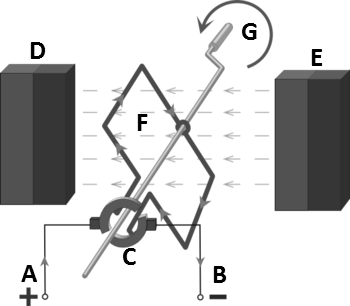
\includegraphics[scale=0.7]{imgs/silnik_p_stalego.png}
 	\caption[Schemat ideowy silnika prądu stałego.]{\small{Rysunek przedstawia ideową budowę szczotkowego silnika prądu stałego, którym możemy wskazać jego poszczególne elementy: A i B - zaciski zasilania, są źródłem prądu płynącego przez ramkę F umieszczoną w polu magnetycznym wytworzonym przez dwa magnesy stałe D i E. Ramka zamocowana jest do osi obrotowej silnika E oraz łączy się z komutatorem C, który jest odpowiedzialny za zmianę kierunku przepływu prądu poprzez zmianę polaryzacji napięcia.}\footnotemark}
	\label{silnik_p}
    \end{center}
  \end{figure}  
  	  \footnotetext{\emph{Silnik prądu stałego}, http://wiki.wolnepodreczniki.pl/,  (data dostępu 28.12.2015 r.)}
\noindent
Sterowanie silnikami odbywa się poprzez zmianę wartości siły $F$. Indukcję magnetyczną $B$ oraz długość przewodu $L$ przyjmuje się jako wartości stałe. Zatem jedynym parametrem, dzięki któremu możliwa jest jej regulacja jest prąd $I$. Dodatkowo zakładając ,że rezystancja ramek wirnika jest zawsze taka sama oraz prawo Ohma (wzór \ref{eq:prawo_ohma}) regulacja upraszcza się do zmiany wartości napięcia zasilającego~$U$. 
\begin{equation}
	I = \frac{U}{R}
   \label{eq:prawo_ohma}
 \end{equation}
 gdzie:  
 \begin{equationDescriptor}
   \EQDitem{$U$}{napięcie [V],}
 	\EQDitem{$R$}{rezystancja [$\Omega$],}
 	 \EQDitem{$I$}{prąd [A],}
 \end{equationDescriptor}
\noindent
Do tego celu wykorzystany został tzw. sygnał PWM, czyli sygnał prostokątny o zmiennym wypełnieniu i określonej częstotliwości (rys. \ref{sygnal_PWM}), którą można obliczyć ze wzoru:
\begin{equation}
	f =  \frac{1}{T}
   \label{eq:czestotliwosc}
 \end{equation}
 gdzie:  
 \begin{equationDescriptor}
   \EQDitem{$f$}{częstotliwość [Hz],}
 	\EQDitem{$T$}{okres sygnału [s].}
 \end{equationDescriptor}
\noindent
 Wypełnienie sygnału definiujemy jako stosunek czasu trwania sygnału do okresu:
 \begin{equation}
	k =  \frac{dT}{T} \cdot 100\%
   \label{eq:wsp_wypelnienia}
 \end{equation}
 gdzie:  
 \begin{equationDescriptor}
   \EQDitem{$dT$}{czas trwania niezerowej wartości sygnału [s],}
 	\EQDitem{$T$}{okres sygnału [s],}
 	\EQDitem{$k$}{współczynnik wypełnienia [\%].}
 \end{equationDescriptor}
 \newpage
  \begin{figure}[H]
    \begin{center}
      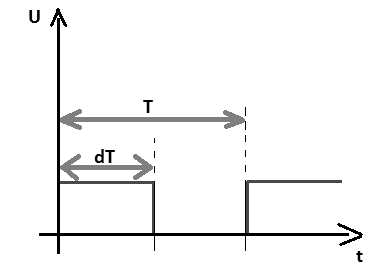
\includegraphics[scale=0.65]{imgs/wykres.png}
 	\caption[Sygnał PWM.]{\small{Na wykresie przedstawiony został przykładowy przebieg PWM, czyli fala prostokątna o okresie $T$ oraz czasie trwania sygnału $dT$.}}
	\label{sygnal_PWM}
    \end{center}
  \end{figure}  
  \noindent
  Wartość wypadkowego napięcia możemy obliczyć ze wzoru:
  \begin{equation}
	U_{sk}=\sqrt{\frac{1}{T}\int\limits_{0}^{dT}u(t)^2dt}
   \label{eq:napiecie_skuteczne}
 \end{equation}
 gdzie:  
 \begin{equationDescriptor}
   \EQDitem{$U_{sk}$}{napięcie skuteczne [V],}
 	\EQDitem{$T$}{okres sygnału [s],}
 	 \EQDitem{$dT$}{czas trwania niezerowej wartości sygnału [s].}
 \end{equationDescriptor}
 
 \namedsection[Adam Zieliński]{Sterowanie wieżyczką}
Serwomechanizm jest kompaktowym urządzeniem mechaniczno-elektronicznym (rys. \ref{serwomechanizm}) składającym się z silnika prądu stałego oraz sterownika. Najczęściej układy tego typu realizują sterowanie położeniem wału wyjściowego i mają ograniczony zakres pracy (np. umożliwiają obrót o 270$^\circ$). Urządzenia posiadają w sobie pętlę sprzężenia zwrotnego (np. przy wykorzystaniu potencjometru połączonego z wałem) oraz zaimplementowany sterownik. 
  \begin{figure}[H]
    \begin{center}
      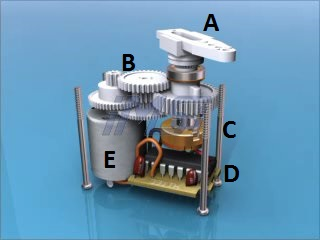
\includegraphics[scale=0.8]{imgs/serwo.jpg}
 	\caption[Model sewomechanizmu.]{\small{Ilustracja przedstawia wewnętrzną budowę serwomechanizmu, na którym: A - orczyk, czyli część obrotowa/wykonawcza, B - zespół kół zębatych redukujących prędkość obrotową, C - potencjometr realizujący sprzężenie zwrotne od położenia orczyka, D - układ elektroniczny będący sterownikiem układu, E - silnik prądu stałego.}\footnotemark}
	\label{serwomechanizm}
    \end{center}
  \end{figure}  
  	  \footnotetext{\emph{Model serwomechanizmu}, http://imsi.pl/,  (data dostępu 28.12.2015r.)}
\noindent
Sterowanie, podobnie jak w przypadku napędu, odbywa się przy wykorzystaniu modulacji szerokości impulsu PWM. Jednakże generowany sygnał musi mieć określoną częstotliwość - 50 Hz a zmiana wypełnienia powoduje zmianę położenia orczyka. Przykładowy sposób sterowania przedstawiony został na rysunku \ref{serwomechanizm_sterowanie}. Dla wypełnienia $k=7,5$\% układ ustawia się w położeniu neutralnym, czyli w połowie zakresu działa - 90$^\circ$ względem początkowego położenia. Zmniejszając stopniowo wypełnienie sygnału sterującego orczyk będzie zmniejszał kąt wychylenia (aż dojdzie do 0 $^\circ$), zwiększając - kąt będzie narastał aż do 180$^\circ$.
\begin{figure}[H]
    \begin{center}
      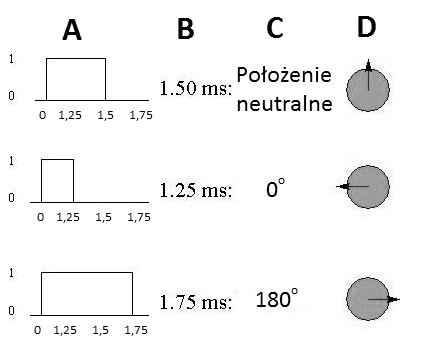
\includegraphics[scale=0.8]{imgs/ster_serw.png}
 	\caption[Sterowanie serwomechanizmem.]{\small{Ilustracja przedstawia przykładowe sterowanie serwomechanizmem. Kolumna A przedstawia sygnał wejściowy o częstotliwości 50 Hz, czyli okresie $T=20$ ms, B - wskazuje nam czas trwania sygnału $dT$, C i D - położenie wału wyjściowego.}\footnotemark}
	\label{serwomechanizm_sterowanie}
    \end{center}
  \end{figure}  
  	  \footnotetext{\emph{Co to jest serwomechanizm?}, http://henryk.mbapp.com/,  (data dostępu 28.12.2015r.)}
  	  
\namedsection[Adam Zieliński]{Magistrala TWI}
Interfejs TWI jest protokołem komunikacyjnym pozwalającym połączyć ze sobą różnego rodzaju układy elektroniczne takie jak mikrokontrolery czy czujniki pomiarowe. Dane przesyłane są szeregowo z wykorzystaniem dwóch linii sygnałowych: SCL (ang. \textit{Serial Clock Line}) oraz SDA (ang. \textit{Serial Data Line}). Do funkcjonowania magistrali nie są wymagane żadne układy zewnętrzne. Należy jedynie zapewnić wysoki stan logicznego (5 V lub 3,3 V) na szynach, co przedstawione zostało na rysunku \ref{podlaczenie_TWI}. Dodatkowo każde z podłączonych urządzeń musi posiadać swój unikalny adres. Wartości rezystorów R1 oraz R2 są odwrotnie proporcjonalne do pojemności pasożytniczej magistrali oraz prędkości przesyłu danych.
\begin{figure}[H]
    \begin{center}
      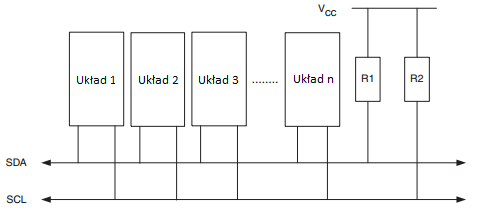
\includegraphics[scale=0.9]{imgs/magistrala_twi.png}
 	\caption[Magistrala TWI.]{\small{Rysunek przedstawia sposób podłączenia urządzeń do wspólnej magistrali TWI. Wymagane jest dołączenie rezystorów podciągających R1 dla SDA i R2 dla SCL dla zapewnienia wysokiego stanu logicznego linii.}\footnotemark}
	\label{podlaczenie_TWI}
    \end{center}
  \end{figure}  
  	  \footnotetext{\emph{Atmega48 datasheet}, http://atmel.com/,  (data dostępu 20.08.2015 r.)}
\newpage
\noindent
Urządzenia mogą pracować w dwóch trybach :
\begin{table}[h!tb]
\centering
\small
\caption{Tryby pracy TWI}
\begin{tabularx}{\linewidth}[c]{|l|X|} 
\hline
	Tryb & Pełniona funkcja \\ \hline
 	\textit{Master} & Urządzenie nadrzędne, może inicjować transmisję, jest odpowiedzialny za generowanie sygnału zegarowego.  \\ \hline
 	\textit{Slave} & Nie może inicjować wymiany danych. Transmisja możliwa jest jedynie w odpowiedzi na sygnał otrzymany od urządzenia typu \textit{Master}, nie może generować sygnału zegarowego.\\ \hline
 	\noalign{\smallskip}
\end{tabularx}
\vspace{-8pt}
\end{table}
\newline
\noindent
Przykładowa wymiana informacji pomiędzy układem \textit{Master} i \textit{Slave} została przedstawiona na rysunku \ref{trans_TWI}. W stanie bezczynności każda z szyn danych ma wysoki stan logiczny. Inicjacja transmisji rozpoczyna się wysłaniem tzw. bitu startu - \ref{trans_TWI}A, czyli wymuszeniem zbocza opadającego linii danych gdy linia zegarowa utrzymuje stan wysoki. Następnie \textit{Master} szeregowo wysyła bajt danych, z czego najstarsze 7 bitów to adres urządzenia docelowego - \ref{trans_TWI}B (stąd do magistrali można podłączyć maksymalnie $2^7$ urządzeń). Najmłodszy bit oznacza realizowaną funkcję : 0 - zapis, 1 - odczyt - \ref{trans_TWI}C. Urządzenie, które poprawnie odczytało swój unikalny adres powinno w odpowiedzi wygenerować bit potwierdzenia - \ref{trans_TWI}D. Następnie rozpoczyna się transmisja danych - \ref{trans_TWI}E. Dane wysyłane są bajtami. Każda odebrana ramka potwierdzana jest bitem potwierdzenia~-~\ref{trans_TWI}F. Transmisja nie definiuje ilości możliwych do wysłania bitów. Trwa ona tak długo, aż nie pojawi się bit stopu, czyli zbocze narastające na linii SDA w momencie ,gdy SCL ma stan wysoki - \ref{trans_TWI}G. Mimo możliwości podłączenia do 128 urządzeń nie możliwe jest prowadzenie wielu transmisji jednocześnie. Największą zaletą TWI jest możliwość podłączenia względnie dużej ilości układów przy wykorzystaniu jedynie dwóch pinów mikrokontrolera. 
\begin{figure}[H]
    \begin{center}
      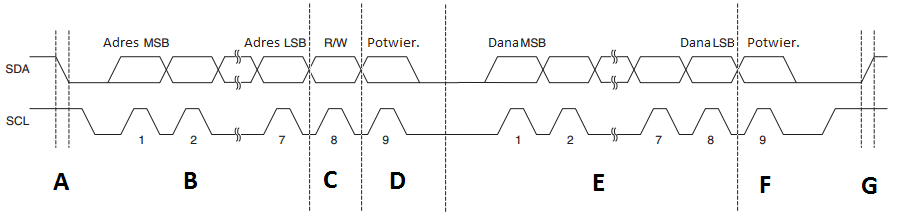
\includegraphics[scale=0.6]{imgs/transmisja_twi.png}
 	\caption[Transmisja TWI.]{\small{Rysunek przedstawia przykładową transmisję danych. Kolejne etapy to: A - bit startu (\textit{Master}), B - wysłanie adresu urządzenia docelowego (\textit{Master}), C - bit oznaczający zapis/odczyt danych (\textit{Master}), D - bit potwierdzenia odbioru generowany przez urządzenie docelowe (\textit{Slave}), E - bajt danych (zapis - \textit{Master} lub odczyt - \textit{Slave}) , F - potwierdzenie odbioru (zapis - \textit{Slave} lub odczyt - \textit{Master}), G - bit stopu (\textit{Master}). MSB (ang. \textit{Most Significant Bit}) - najbardziej znaczący bit, LSB (ang. \textit{Least Significant Bit}) - najmniej znaczący bit. }\footnotemark}
	\label{trans_TWI}
    \end{center}
  \end{figure}  
  	  \footnotetext{\emph{Atmega48 datasheet}, http://atmel.com/,  (data dostępu 20.08.2015 r.)}	
  	  
\namedsection[Adam Zieliński]{Sterownik silników}
Silniki napędowe wyposażone są w enkodery impulsowe, czyli  urządzenia które generują (w tym przypadku) około 370 impulsów na jeden, pełny obrót koła. Jest to wystarczające źródło informacji, na podstawie którego można określić prędkość obrotu silnika a następnie zaprojektować regulator prędkości. Sterownik zrealizowany jest przy wykorzystaniu  mikrokontrolerów z rodziny AVR, Atmega48. Jest to 8-bitowy układ oparty na architekturze RISC (ang. \textit{Reduced Instruction Set Computing} – polega on przede wszystkim na uproszczeniu listy rozkazów, składającej się w większości z poleceń wykonywanych w jednym takcie zegara, co umożliwia szybsze wykonywanie kodu) oraz architekturze harwardzkiej, w której to pamięć danych programu jest oddzielona od pamięci rozkazów. Jednostka ta jest wyposażona w sprzętowe generatory sygnałów PWM oraz liczniki pozwalające zliczać sygnały z enkoderów - co w pełni spełnia nasze wymagania. Dodatkowo układy AVR wspierają także komunikację wykorzystującą protokół TWI - co zapewnia nam pełną integrację z \textit{Raspberry Pi}.

\namedsection[Adam Zieliński]{Zasilanie}
Aby projektowany pojazd był w pełni mobilny należy zapewnić mu przenośne źródło zasilania - baterię. Ze względu na fakt, iż robot powinien możliwie długo pracować autonomicznie zastosowana została bateria 
